\documentclass[tikz,border=5pt]{standalone}
\usepackage{amsmath}
\definecolor{accent}{HTML}{5A3C67}
\definecolor{tint}{HTML}{EDE6F2}
\begin{document}
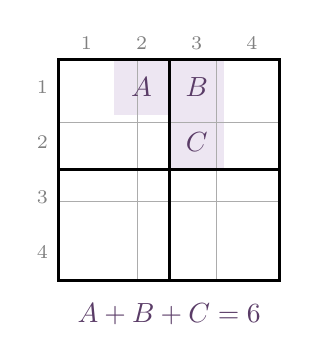
\begin{tikzpicture}[x=.7cm,y=.7cm,font=\sffamily]
  \ifdefined\Practice
    \foreach \r/\c in {2/2,3/2,3/3} {\fill[tint] (\c-1,4-\r) rectangle +(1,1);}
  \else
    \foreach \r/\c in {1/2,1/3,2/3} {\fill[tint] (\c-1,4-\r) rectangle +(1,1);}
  \fi
  \draw[gray!65,thin] (0,0) grid (4,4);
  \draw[line width=1.1pt] (0,0) rectangle (4,4);
  \draw[line width=1.1pt] (2,0)--(2,4) (0,2)--(4,2);
  \foreach \i in {1,...,4} {
    \node[gray,font=\scriptsize] at (\i-.5,4.3) {\i};
    \node[gray,font=\scriptsize] at (-.3,4.5-\i) {\i};
  }
  \ifdefined\Practice
    \node[accent] at (1.5,2.5) {$A$};
    \node[accent] at (1.5,1.5) {$B$};
    \node[accent] at (2.5,1.5) {$C$};
    \node[anchor=north,accent] at (2,-.25) {$A+B+C=9$};
  \else
    \node[accent] at (1.5,3.5) {$A$};
    \node[accent] at (2.5,3.5) {$B$};
    \node[accent] at (2.5,2.5) {$C$};
    \node[anchor=north,accent] at (2,-.25) {$A+B+C=6$};
  \fi
\end{tikzpicture}
\end{document}
